\section{Soil Erosion Processes}
\label{sec:SoilErosionProcesses}

%\subsection{Introduction}
%\label{sec:ErosionProcessesIntroduction}

\begin{quote}
  \begin{quote}
    ``Erosion by water is the redistribution and removal of the
upper layers of the soil, both by the action of falling rain, and by water
flowing over the soil during and after rain or following snowmelt.''
\citep{favis-mortlock2002-452}
  \end{quote}
\end{quote}

The erosion of soil by water and wind is a naturally occurring process, which is
commonly accelerated by human activity. However, when soil erosion occurs at a
greater rate than the rate of soil formation, soil erosion is considered as an
environmental problem. Soil erosion is a ubiquitous problem that threatens an
important and non-renewable resource such as the agricultural land that is
suitable for cultivation (on-site impact) \citep{boardman2003-176}. In addition
to removing a valuable resource, soil erosion leads to increased sediment input
to nearby watercourses, resulting in, for example, the silting-up of dams and
contamination of drinking water (off-site impact)
\citep{mejia1994-331,kitchen1998-179}.

Soil erosion problems can be viewed in three different ways
\citep{kirkby1980-312}. Firstly, in the broadest view, soil erosion can be
compared with other processes of landscape denudation. When and where it is the
most rapid process, soil erosion should be recognised as the dominant problem.
This view leads to the question of what erosion rates can be tolerated in the
long-term. Secondly, a narrower overview examines soil erosion with its
immediate climatic and vegetational controls. This then leads to the question as
to how well the processes involved in raindrop impact, flow generation, and
sediment resistance are understood. Thirdly, soil erosion can be studied in
relation to its variable distribution patterns in time and space. The reasons
for the temporal and spatial distributions of soil erosion are however only
partially understood \citep{quine2002-55,gomez2005-143,wakiyama2010-993}.

Soil erosion by water is most active where rainfall cannot infiltrate the soil,
but flows over the surface. As the flow travels down a hillslope, it is able to
carry soil materials away mainly by shear stress although other sub-processes
also contribute \citep[see also Figure
\ref{fig:kinnell}]{kinnell2000-discourse,kinnell2005-2815}. In some
cases, only an hour or two of contact time with the surface soil is needed to
carry away an appreciable amount of material. Thus, where overland flow is
dominant, soil erosion by water is likely to be the main process of landscape
denudation. When a large depth of water flows rapidly over the surface with
correspondingly large hydraulic forces, soil erosion acts catastrophically.
These conditions are most commonly found in semi-arid areas, but fields cleared
for agricultural purposes are also subjected to erosion in almost any climate,
which can on occasion be severe \citep{boardman2001-346,boardman2003-176}.

Semi-arid areas are very sensitive to small natural changes in climate and in
such areas it is difficult to separate natural from man-induced changes in
erosion rates. However, even in temperate-humid areas increased erosion
resulting from farming can be sensitively dependent on the extent of the change
in vegetation cover, the total rainfall at periods of low cover, and the
intensity of the rains.

Therefore, two distinct types of areas appear to be at great risk of soil
erosion. The first is a semi-arid area, and the second is a temperate area that
have been stripped of vegetation for crop cultivation. A soil erosion rate can
reach its maximum where intense rainfall occurs during the period of lowest
vegetation cover. This is normally the case in semi-arid climates or in
temperate areas which have been left bare at the time of the heaviest annual
rainfall \citep{goff1993-698,nearing2005-131}. In such cases, when the rainfall
increases, soil loss increases, so that the erosional peak tends to be
synchronised with the rainfall peak and this relationship becomes more
distinctive when the soil becomes more unprotected
\citep{goff1993-698,nearing2005-131}.

When soil erosion problem is to be considered, it also is worthwhile to take
long-term effects of soil erosion into account. For example, when soil erosion
occurs at a rate of one millimetre per year, it might not have apparent effect
in a human lifetime. However, over a longer-term, the effect can be
considerable. To put this into perspective, topsoil of 15 cm thickness in
general would be completely removed after 150 years if erosion rates stay as
high as 1 mm/year in average with no additional soil formation in the area.
Topsoil contains a high proportion of soil organic matter and the finer mineral
fractions, which provide water and nutrient supplies for plant growth. This may
look like an oversimplification of the erosion process and soil formation, but
it gives us an idea of the long-term effect of soil erosion.

%When soil erosion occurs at a rate of, for example, one millimetre per year, it
%might have little apparent effect in a human lifetime. However, over a
%longer-term, effects can be considerable. This is because erosion continually
%removes the topsoil (e.g., topsoil of 15 cm thickness would be completely
%removed after 150 years if erosion rates are higher as 1 mm/year without
%renewal) which contains a high proportion of soil organic matter and the finer
%mineral fractions, which provide water and nutrient supplies for plant growth.

\subsection{Rainfall}
\label{sec:RainfallCharacteristics}

\subsubsection{Raindrop Splash}
% Raindrop Impact Induced Erosion (need to put more appropriate title)
\label{sec:RaindropSplash}

The process of erosion by water is a two-phase process: detachment and transport
\citep{morgan1995-soil}. Individual soil particles are detached from the soil
mass by the impact of raindrops. The erosive power of raindrops weakens and
loosens the soil surface, and flowing water transports the soil particles
\citep{kinnell2000-discourse}. When sufficient transporting energy is no longer
available, a third phase, deposition, can occur.

\begin{figure}[htbp]
  \centering
  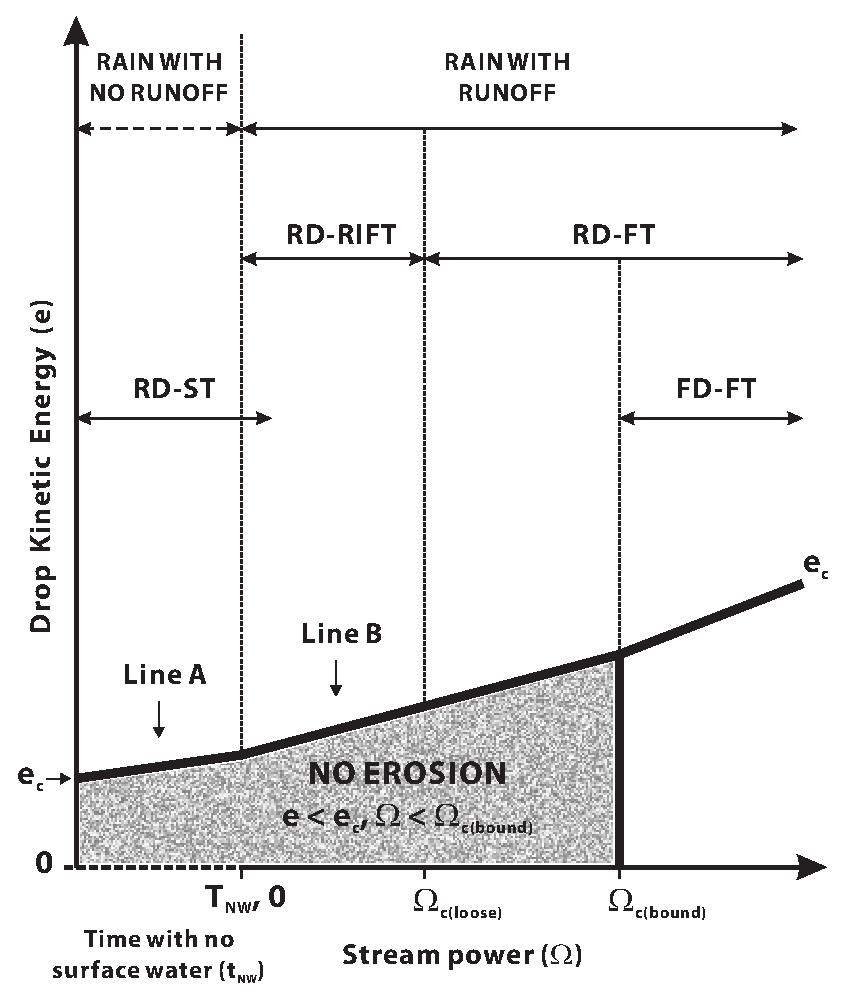
\includegraphics[width=0.70\textwidth]{./img/kinnell}
  \caption[Detachment and transport processes]{Detachment and transport
processes associated with variations in raindrop and flow energies. $T_{NW}$:\
total time when rain falls and there is no surface water. $e_c$:\ critical
raindrop energy to cause detachment; raindrop-induced erosion occurs when drop
energy is equal or greater than $e_c$. Line A:\ $e_c$ when raindrops are
detaching soil particles from the soil surface prior to flow developing. The
slope on this line is used to indicate increasing resistance to detachment
caused by, for example, crust development. Line B:\ $e_c$ when raindrops are
detaching soil particles from the soil surface when flow has developed. The
slope on this line is used to indicate increasing utilization of raindrop energy
in penetrating the flow when flow depth increases as flow power increases.
$\Omega_{c\textrm{(loose)}}$:\ critical stream power required to transport loose
(pre-detached) soil particles. $\Omega_{c\textrm{(bound)}}$:\ critical stream
power required to detach particles bound within the soil surface (held by
cohesion and interparticle friction). RD-ST:\ raindrop detachment and splash
transport. RD-RIFT:\ raindrop detachment and raindrop-induced flow transport.
RD-FT:\ raindrop detachment and flow transport. FD-FT:\ flow detachment and flow
transport\citep[From][]{kinnell2005-2815}.}
  \label{fig:kinnell}
\end{figure}

Raindrop splash distributes soil particles radially away from the site of
detachment. The raindrop detachment-splash transport (RD-ST in Figure
\ref{fig:kinnell}) process is effective where rainfall intensities are high, for
example, as a result of convective rainstorms. However, splash transport (ST) is
a generally inefficient transport mechanism. If the soil has virtually no slope,
soil particles splashed away from the point of impact are replaced by soil
particles detached by other raindrops in the surrounding area
\citep{kinnell2000-discourse,zartl2001-25}. Even if the soil surface has a
slope, net downslope transport by raindrop splash alone is generally small
\citep{kinnell2001-749}.

When water flows start to build up, the soil surface becomes protected from
direct raindrop impact, and another transport mechanism begins to dominate.
Raindrops with sufficient kinetic energy to penetrate through the flow may
detach and lift soil particles into the flow, which then carries them downstream
until it loses sufficient transporting energy to carry the particles. Soil
particles transported by the flow then fall back to the soil surface of lower
grounds. This transport process is termed Raindrop-Induced Flow Transport (RIFT
in Figure \ref{fig:kinnell}) \citep{kinnell1990-497}. While RIFT is more
efficient than ST, it still requires numerous raindrop impacts to move soil
particles downstream.

As rain continues, thin surface water flows become capable of moving loose soil
material on the top of the surface, but might not be capable of detaching soil
material from the soil mass. In many cases, soil particles are detached by the
help of raindrop impacts, and carried away downstream without the need for
raindrops to be involved in the transport process. This raindrop detachment-flow
transport (RD-FT) process is more efficient than RD-RIFT. In a typical field,
both RD-RIFT and RD-FT occur simultaneously in the same flows.

When the critical stream power ($\Omega_{c\textrm{(bound)}}$) for flow to detach
soil particles from soil mass exceeds stream power ($\Omega$), flow detachment
(FD) occurs \citep{kinnell2000-discourse}. Once soil materials are detached and
transported by flow (FD-FT), erosional channels are generated (Figure
\ref{fig:kinnell}). As these channels develop and increase in size to become
large rills and possibly even gullies, processes such as gravitational collapse
of channel walls and heads become important \citep{boardman2003-165}.

\subsubsection{Rainfall Intensity} % Rainfall Intensity Patterns?
\label{sec:RainfallIntensity}

The erosive power of rainfall has long been appreciated by studies on soil
erosion \citep{musgrave1947-133,wischmeier1958-rainfall}. Nevertheless,
obtaining information on rainfall intensity for soil erosion is very much
problematic. One way of measuring rainfall intensity would be measuring size,
distribution and velocity of raindrops, so that the kinetic energy of the
rainfall can be calculated \citep{cerda1997-169,lascelles2000-709}. This can be
seen as a `bottom-up' approach. Another method would be simply to measure
rainfall amount and duration, so that intensity can be obtained by dividing
rainfall amount by duration (i.e. rainfall amount per unit time)
\citep{osborn1998-505}. This is a `top-down' approach. However, both approaches
have their own shortcomings
\citep{parsons2000-723,schuur2001-1019,garcia2001-675}.

Although rainfall intensity plays a very important role for soil erosion, it is
important to recognise that the vital variable for soil erosion by splash is not
rainfall intensity itself, but rainfall energy. This rainfall energy varies in
association with rainfall intensity. As raindrops increase in size, their
terminal velocity increases. This increases the kinetic energy of raindrops. The
total kinetic energy of rainfall also increases with increasing number of
raindrops during a given time. The total kinetic energy of rainfall may be
estimated from the distribution of raindrop size and number of raindrops during
a storm. The accuracy of this estimation is, however, limited by natural
variations in rainfall characteristics \citep{vandijk2002-1}. Yet, in natural
rainfall events, the relationship between rainfall intensity and energy is
neither so clear, nor simple. Despite this, simple assumptions about the
rainfall intensity-energy relationship are often made in studies on soil
erosion, in particular, modelling studies, as rainfall intensity is the
only easily modifiable control on rainfall energy in such studies
\citep{laflen1997-96,morgan1998-389}.

\citet{parsons2006-68} ran a laboratory-based rainfall simulation
experiment to determine the implications of temporal variation of rainfall
intensity for rates of soil loss. They found that erosion is least for the
constant-intensity storms. This is highly significant because soil-erosion
models are typically calibrated using data obtained from constant-intensity
experiments. Moreover, storm pattern does not appear to affect the volume of
runoff, but it does affect the quantity of eroded sediment. In particular, the
constant-intensity storm patterns are associated with low erosion rates. Storm
pattern also affects the size-distribution of the eroded sediment.
\citet{parsons2006-68} therefore concludes that the relationship between
rainfall energy and interrill erosion is more complex than is currently assumed
in process-based models of soil erosion.

Other studies also note that there are complex interactions between raindrop
size, velocity and the duration of rain, which control the erosive power of
rainfall \citep{kinnell1981-153,brandt1990-687,salles1999-545,vandijk2002-1}.

\subsection{Soil Type}
\label{sec:SoilType}

Soil erodibility is an estimate of the resistance of the soil to erosion, based
on the physical characteristics of each soil \citep{morgan1995-soil}. Although
erodibility varies with soil texture, aggregate stability, shear strength,
infiltration capacity and organic and chemical contents, soils with high
infiltration rates, higher levels of organic matter and improved soil structure
have a greater resistance to erosion, in general \citep{morgan1995-soil}.

Erodible soils have restricted clay content \citep{bryan2000-385}. Soils with
more than 30--35\% clay are generally coherent and form stable soil aggregates,
which are resistant to raindrop impact and splash erosion
\citep{evans1980-mechanics}. Clays often have rough surfaces to store much
water, and are resistant to sheet and rill erosion. Sands and coarse loamy
sands, on the other hand, have high infiltration rates and resistant to erosion,
and even if this is exceeded, sands (more than 0.3 mm diameter) are not easily
eroded by flowing water or by raindrop impact
\citep{evans1980-mechanics,marshall1996-soil}.

Sandy soils are however more erodible than clayey soils because the aggregates
of these sandy soils slake more readily and seal the soil surface
\citep{lebissonnais1996-425}. Loamy soils are also particularly at risk of
sealing \citep{ramos2000-398}.

After cultivation, the soil surface becomes rough. The amount of water, which
can be stored on the surface before runoff takes place, is thus large at this
time. Surface roughness is least after drilling and rolling of the seedbed, and
differences between soil types are smallest \citep{robinson1992-151}. For
similar soil types, the timing of cultivation can affect the storage volume, for
example, a clay surface prepared in winter can have more than twice as much
storage volume as a surface prepared in spring \citep{evans1980-mechanics}.

Moreover, stony soils are generally less vulnerable to erosion as the surface
stones not only protect the soil, but also increase infiltration by providing
larger pores between stones
\citep{agassi1991-565,poesen1994-1,defigueiredo1998-81}. However, when rock
fragments are well-embedded in a surface seal, a positive relation for runoff
and sediment yield is found \citep{poesen1992-451}. A negative relation occurs
either where rock fragments are partly embedded in a top layer with structural
porosity or where the rock fragments rest on the surface of a soil having either
textural or structural pore spaces \citep{poesen1992-451}.

\subsection{Topography}
\label{sec:Topography}

There are two aspects of topography that affect erosion: slope angle and length.
Normally, erosion would be expected to increase as the slope steepness increases
\citep{liu1994-1835}. Soil erosion by water also increases as the slope length
increases because of increases in velocity and volume of runoff
\citep{liu2000-1759}. Water depth increases with downslope distance so that
interrill soil erosion is affected by slope length \citep{gilley1985-154}.
Water depth then affects soil detachment and overland flow sediment transport
capacity \citep{gilley1985-147}. Slope angle is also closely related to the
effectiveness of splash erosion \citep{kinnell2000-discourse,vandijk2003-153}.

Overall slope orientation and steepness are major factors that control the
location and development of hillslope rills.
%The location of downslope is an important factor that determines the
%development of rills on a hillslope.
However, there is another factor that is closely related to the dynamics of
initiation and growth of rills. The minute variations of soil surface
topography, also known as microtopography, can play an  important roll on this
``rill competition''.

Microtopography is not temporally static because erosional processes will
continuously modify the surface of soil during a rainfall event. As a
result, runoff during the latter part of the event will flow over a soil
surface that has been modified and different from the surface earlier in the
rainfall. Thus, erosive modification of microtopography constitutes a feedback
loop which might be expected to operate in a positive sense. The most
`successful' rills (i.e. those conveying the most runoff) will modify the local
microtopography to the greatest extent, and so will most effectively increase
their chances of capturing and conveying subsequent runoff.

\citet{favis-mortlock2000-2173} previously recognised the importance of
microtopography in the initiation and the development of rills, and developed a
erosion model, RillGrow, using a self-organising dynamic systems approach. More
about RillGrow is included in Section \ref{sec:ModelDescriptionRillGrow}.
%******you need to mention also something about microtopograghy, at the mm to cm
%scale, about how this is important in (among other things) determining the
%location of preferential flow paths and so of rills.

\subsection{Land Use}
\label{sec:LandUse}

Soil erosion potential is highest where the soil has no or very little
vegetative cover. Vegetation cover protects the soil from direct raindrop impact
and splash, and tends to slow down surface runoff. On a field with complete
vegetation cover, runoff and erosion are comparatively small, often less than
5\% of runoff and 1\% of erosion from bare soil, respectively
\citep{braskerud2001-1447,rey2003-549}. One reason is because the infiltration
rates of the vegetated field are relatively higher than those on bare soils as
the field often has a better soil structure and more stable aggregates
\citep{robinson2001-1}. When runoff does take place, the leaves and roots of
plants inhibit the flow by reducing the velocity of the flow
\citep{braskerud2001-1447,rey2003-549}. On soils with less than 70\% vegetation
cover, runoff and erosion increase rapidly when rainfall occurs
\citep{favis-mortlock1996-529}. Under less than 20--30\% vegetation cover,
runoff and erosion are related to the amount of bare ground, increasing as the
proportion of bare ground increases \citep{favis-mortlock1996-529}.

The effectiveness of any crop management system against soil erosion by water
also depends on how much protection is available at various periods during the
year, relative to the rainfall amount that falls during these periods. In this
respect, crops which cover for a major portion of the year (e.g., alfalfa or
winter cover crops) can reduce erosion much more than can crops (e.g., row crops
) which leave the soil bare for a longer period of time and particularly during
periods of intense rainfall \citep{zhang1995-1069,zhang1995-1079}.

%\subsection{Rill and Interrill Erosion}
%\label{sec:RillAndInterrillErosion}
%
%Rills are initiated at a critical distance downslope where overland flow
%becomes channelled.
%
%Interrill erosion is due to detachment and transport by raindrop impact and
%overland flow. Interrill erosion has been shown to be approximately
%proportional to the square of the rainfall intensity \citep{watson1986-97}.
%In addition to rainfall intensity, interrill erosion is related to slope
%\citep{watson1986-97}.
